\documentclass[tikz,border=2pt]{standalone}
\usepackage{amsmath,amssymb}
\usetikzlibrary{arrows.meta,decorations.pathreplacing}
\begin{document}
% Prospective view at duration t (policy in force): only cash flows after t count, valued at t.
% Expected future benefits and expenses 50 minus expected future premiums 30 gives V_t = 20.
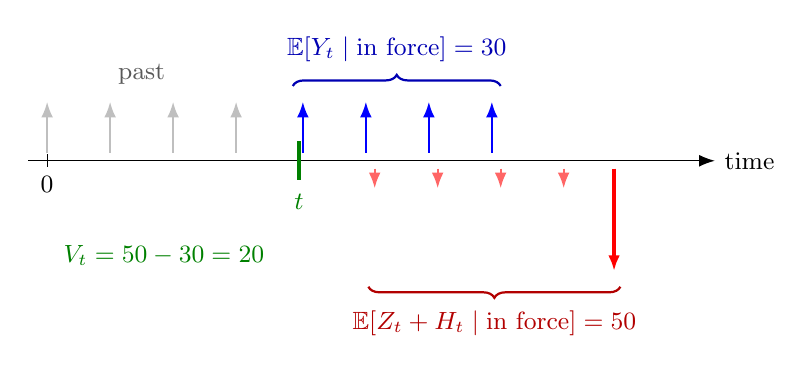
\begin{tikzpicture}[font=\small, >={Latex[length=2mm]}, x=0.8cm]
  \draw[->] (-0.3,0) -- (10.6,0) node[right] {time};
  \draw (0,0.08) -- (0,-0.08) node[below] {$0$};
  \draw[green!50!black, very thick] (4,0.25) -- (4,-0.25);
  \node[green!50!black, anchor=north] at (4,-0.3) {$t$};
  % past premiums (already paid, ignored)
  \foreach \k in {0,1,2,3} \draw[->, gray!50, thick] (\k,0.1) -- (\k,0.75);
  \node[gray!70!black, anchor=south] at (1.5,0.85) {past};
  % future premiums
  \foreach \k in {4,5,6,7} \draw[->, blue, thick] (\k+0.06,0.1) -- (\k+0.06,0.75);
  % future benefit and expenses
  \foreach \k in {5,6,7,8} \draw[->, red!60, thick] (\k+0.2,-0.1) -- (\k+0.2,-0.35);
  \draw[->, red, very thick] (9,-0.1) -- (9,-1.4);
  \draw[blue!70!black, thick, decorate, decoration={brace, amplitude=4pt}]
    (3.9,0.95) -- (7.2,0.95) node[midway, above=5pt] {$\mathbb E[Y_t\mid\text{in force}]=30$};
  \draw[red!70!black, thick, decorate, decoration={brace, mirror, amplitude=4pt}]
    (5.1,-1.6) -- (9.1,-1.6) node[midway, below=5pt] {$\mathbb E[Z_t+H_t\mid\text{in force}]=50$};
  \node[green!50!black, anchor=north east] at (3.6,-0.95) {$V_t=50-30=20$};
\end{tikzpicture}
\end{document}
